\chapter{多大语言模型系统中基于角色的交互}\label{chap:roleint}\label{chap:role}

\begin{learningbox}
本章将介绍多个大语言模型（large language model，LLM）智能体在被赋予角色并安排在群体中交互时，会表现出怎样的行为。具体而言，学完本章后，你将能够：
\begin{itemize}[leftmargin=*, nosep]
    \item 区分{\em 基于角色的}多智能体交互（本章）与{\em 开放式}涌现模拟（第~\ref{chap:emergent}~章）。
    \item 描述大语言模型智能体在{\em 博弈论}情境中相互交互时的行为，并将其与单智能体的策略行为研究结果联系起来（第~\ref{chap:behavior}~章）。
    \item 解释{\em 基于角色的协作模式}，并识别实现这些模式的框架。
    \item 批判性地评估多智能体协作何时能够改善表现、何时不能，以及多智能体交互会引入哪些新的失效模式和{\em 安全风险}。
\end{itemize}
\end{learningbox}

\section{从单智能体到多智能体}
上一章从行为的视角研究了单个大语言模型及由大语言模型驱动的智能体：单个模型如何理解交流、社会或道德情境，并在其中行动。本章将从单智能体情境转向多智能体情境，考察多个基于大语言模型的智能体被安排相互交互时会发生什么，例如让它们在博弈论竞赛中互为对手，或在团队中充当协作者。分析单位也随之从单个模型的行为特征，转变为模型之间产生的交互模式与集体结果。

\subsection{多智能体模拟：历史与现状}
在计算社会科学（computational social science）中，利用人工智能体研究交互有着悠久的历史 \citep{epstein1996growing,macal_tutorial_2010}。传统上，具备基本感知、推理与决策能力的智能体群体，在虚拟实验环境中进行交互；若模拟以机器人为基础，则是在真实实验环境中交互 \citep{steels1995self,shoham2008multiagent}。这类模拟通常旨在连接理论研究与实验研究：对于难以开展现实实验或实验成本高昂的领域，利用人工行为来检验有关人类行为的假设。

历史上，这一研究方向一直受到两大障碍的限制：难以验证行为是否符合现实，以及模拟智能体社会所需的高昂计算成本。智能体大语言模型与模拟基础设施的进步 \citep{rutherford2024jaxmarl} 正在改变这种状况。基于大语言模型的智能体能够用自然语言交流、处理丰富的背景知识，还可以被赋予不同的角色设定（persona）。这些能力使模拟交互的表达更加丰富，也更便于直接与人类交互进行比较。

\subsection{基于角色的交互与涌现交互}
我们可以根据研究者对模拟的控制程度，对多大语言模型研究进行分类。在这一连续谱的一端，每个智能体都被赋予一个\emph{角色}，其具体形式包括角色设定、目标与交互协议。研究问题通常是：智能体在指定结构内如何行动，以及与其他指定结构和角色相比，所形成的系统整体表现如何。在另一端，智能体被置于开放式环境中，事先不分配角色；研究问题则是会\emph{涌现}出怎样的社会结构，例如群体动态、惯例与规范。本章关注这一连续谱中基于角色的一端，第~\ref{chap:emergent}~章讨论涌现的一端。

这一区别对方法选择和结果解释都很重要。在基于角色的系统中，角色与交互协议属于设计决策或实验变量。行为的评估与解释以系统的设计目标为依据。在涌现情境中，目标或任务处于背景位置，甚至完全不存在。分析更为开放，也更具探索性，相比基准测试，更接近民族志。不过，正如后文将会说明的，这一区分并不绝对：基于角色的系统也经常表现出其设计之外的行为。

\subsection{多智能体协作的五个维度} \label{fivedimensions}
为了组织本章内容，我们采用 \citet{tran2025multi} 提出的分类，从五个维度考察大语言模型协作：
\begin{enumerate}
    \item \emph{参与者}：参与交互的智能体，以及它们是同质的（同一模型的多个实例），还是异质的（不同的模型或能力配置）。
    \item \emph{交互类型}：合作、竞争，或两者的混合，即“竞合（coopetition）”。
    \item \emph{结构}：智能体如何组织，例如点对点、集中式或分布式。
    \item \emph{策略}：如何引出协作，例如通过角色分配，或通过模型层面的机制。
    \item \emph{协调协议（coordination protocol）}：将智能体联系起来并规范其通信的机制。
\end{enumerate}
本章讨论的系统在这五个维度上作出了不同选择。记住这些维度，有助于看清各个框架的新意所在。

\subsection{方法论说明}
评估多智能体系统，会继承评估单个模型时的所有方法论困难：提示敏感性、测试材料可能泄漏到训练数据中，以及采样变异。此外，它还会带来一些新的困难：
\begin{itemize}
    \item 报告中的结果往往更难复现，因为一个智能体输出中的细微变化会沿着后续交互级联传播，增大不同运行之间的变异。
    \item 表现差异的成因可能并不明确：究竟是多智能体协作本身、协调协议、为角色分工而嵌入的提示工程，还是仅仅因为多个智能体累计消耗了更多推理预算？
    \item 构念效度（construct validity）问题转移到了社会交互术语层面：{\em 团队合作}、{\em 讨论}或{\em 集体决策（collective decision-making）}等概念带有丰富的人类行为内涵，而实际模拟未必足以支持这些内涵。
\end{itemize}
带着这些限定，本章将首先讨论最简单的多智能体情境：大语言模型智能体在策略情境中彼此交锋，除了博弈本身要求的角色之外，不再分配其他角色（第~\ref{sec:strat}~节）。随后，我们考察通过定义协调协议与明确角色来组织交互之后，会发生什么变化（第~\ref{sec:roletask}~节）。

\section{大语言模型智能体之间的策略交互} \label{sec:strat}
在第~\ref{chap:behavior}~章中，我们考察了大语言模型在提示下与按脚本行动的对手进行经济博弈时的行为。这里，我们讨论{\em 大语言模型智能体彼此交互}的博弈论情境。本节中的智能体是地位对称的同伴：各自追求自身利益，没有任何智能体被赋予协调或监督角色。我们先看同时在多种博弈中为大语言模型智能体评分的基准测试，再看围绕单一情境构建、内容更丰富的模拟平台中的行为。

\subsection{跨博弈的策略能力基准测试}
MAgIC 研究 \citep{xu2024magic} 使用了社交推理游戏（social deduction game，如 Undercover 与 Chameleon），以及成本分摊、多玩家囚徒困境（Prisoner's Dilemma）和公共物品博弈（public goods game）等博弈论情境。其目标是提取七项能力：理性、判断、推理、欺骗、自我意识、合作与协调，如图~\ref{fig:radar}~所示。研究在多智能体情境中，评估现成及增强版大语言模型的这些能力。

GPT-o1 与 GPT-4 的得分显著高于其他模型。总体而言，大语言模型在判断、理性与合作方面得分较高，一些模型在欺骗方面也得分较高；但它们的推理得分较低，协调得分则除一个模型外都较低。唯一的例外是使用概率图建模（probabilistic graphical modeling）增强的 GPT-o1。这种方法受到 \citet{kollerfriendman2009pgm} 的启发，实现了一种类似心智理论（theory of mind，ToM）的能力。作者表明，概率图建模能够全面提升大语言模型的表现。这与第~\ref{sec:theoryofmind}~节讨论的总体证据一致：人类在策略情境中高度依赖心智理论。

\begin{figure}
  \begin{center}
    \begingroup
\linespread{1}\selectfont
\resizebox{\linewidth}{!}{%
\begin{tikzpicture}[x=1pt,y=-1pt]
\node[anchor=north west,inner sep=0pt,outer sep=0pt] at (0,0) {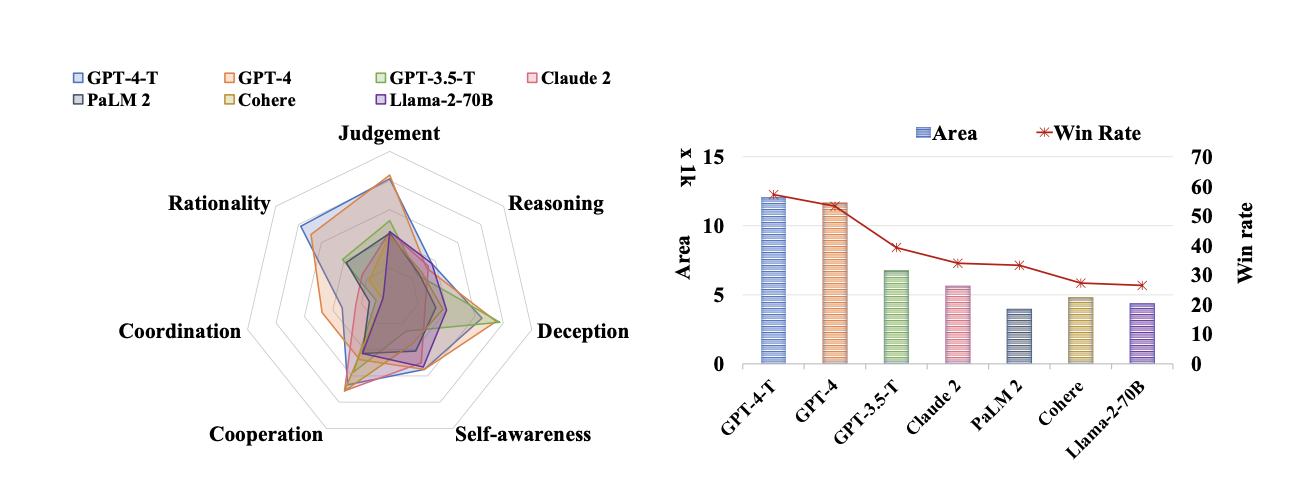
\includegraphics[width=1294pt]{figures/radar.png}};
\fill[fill=white] (335,119) rectangle (452,147);
\node[anchor=center,inner sep=0pt,outer sep=0pt,align=center,text width=111pt,text=black,font={\fontsize{27.7286}{31.6106}\selectfont\sffamily\bfseries}] at (393.5,133) {判断};
\fill[fill=white] (506,190) rectangle (617,218);
\node[anchor=center,inner sep=0pt,outer sep=0pt,align=center,text width=105pt,text=black,font={\fontsize{27.7286}{31.6106}\selectfont\sffamily\bfseries}] at (561.5,204) {推理};
\fill[fill=white] (536,318) rectangle (654,347);
\node[anchor=center,inner sep=0pt,outer sep=0pt,align=center,text width=112pt,text=black,font={\fontsize{27.7286}{31.6106}\selectfont\sffamily\bfseries}] at (595,332.5) {欺骗};
\fill[fill=white] (450,420) rectangle (604,449);
\node[anchor=center,inner sep=0pt,outer sep=0pt,align=center,text width=148pt,text=black,font={\fontsize{27.7286}{31.6106}\selectfont\sffamily\bfseries}] at (527,434.5) {自我意识};
\fill[fill=white] (205,420) rectangle (354,450);
\node[anchor=center,inner sep=0pt,outer sep=0pt,align=center,text width=143pt,text=black,font={\fontsize{27.7286}{31.6106}\selectfont\sffamily\bfseries}] at (279.5,435) {合作};
\fill[fill=white] (112,318) rectangle (242,348);
\node[anchor=center,inner sep=0pt,outer sep=0pt,align=center,text width=124pt,text=black,font={\fontsize{27.7286}{31.6106}\selectfont\sffamily\bfseries}] at (177,333) {协调};
\fill[fill=white] (164,190) rectangle (273,218);
\node[anchor=center,inner sep=0pt,outer sep=0pt,align=center,text width=103pt,text=black,font={\fontsize{27.7286}{31.6106}\selectfont\sffamily\bfseries}] at (218.5,204) {理性};
\fill[fill=white] (931,121) rectangle (999,146);
\node[anchor=center,inner sep=0pt,outer sep=0pt,align=center,text width=62pt,text=black,font={\fontsize{26.5732}{30.2935}\selectfont\sffamily\bfseries}] at (965,133.5) {面积};
\fill[fill=white] (1053,121) rectangle (1150,146);
\node[anchor=center,inner sep=0pt,outer sep=0pt,align=center,text width=91pt,text=black,font={\fontsize{26.5732}{30.2935}\selectfont\sffamily\bfseries}] at (1101.5,133.5) {胜率};
\fill[fill=white] (669,229) rectangle (702,285);
\node[anchor=center,inner sep=0pt,outer sep=0pt,align=center,text width=27pt,text=black,font={\fontsize{25.129}{28.6471}\selectfont\sffamily\bfseries}] at (685.5,257) {面\\积};
\fill[fill=white] (1232,199) rectangle (1263,288);
\node[anchor=center,inner sep=0pt,outer sep=0pt,align=center,text width=25pt,text=black,font={\fontsize{25.129}{28.6471}\selectfont\sffamily\bfseries}] at (1247.5,243.5) {胜\\率};
\pgfresetboundingbox
\path[use as bounding box] (0,0) rectangle (1294,494);
\end{tikzpicture}}
\endgroup

    \caption{大语言模型在不同指标上的表现 \citep{xu2024magic}}\label{fig:radar}
  \end{center}
\end{figure}

LLM-Coordination Benchmark \citep{agashe2025llm} 则将协调单独作为研究对象，而不是把它当作多个特质之一。该基准测试在两项不同任务上评估大语言模型：纯合作博弈中的智能体协调，以及针对这些博弈的问答（见图~\ref{fig:agashe}）。实验发现，只要决策能够依赖环境变量，大语言模型智能体就表现良好；但当成功需要主动推理同伴的信念与意图时，它们的表现就很差。具体而言，这些环境变量包括游戏布局、物体位置、每个智能体当前所在的位置、哪些门已经打开等。最清楚的例子是 Overcooked-AI，这也是大语言模型表现最好的游戏。该游戏完全可观测，其动作空间包含{\em 从洋葱供应器 1 取一个洋葱}、{\em 将洋葱放在盘子 0 上}等动作。在大多数情境与布局下，大语言模型只需根据游戏环境的状态，考虑下一步的最佳动作，而无须考虑其他智能体的视角。

将 Overcooked 的表现与 Hanabi 的得分进行比较时，这种不对称性尤为明显。在 Hanabi 中，每个动作都需要推理同伴的信念。在 Overcooked 中，零样本大语言模型智能体能够达到或超过专门训练的强化学习基线模型的表现。然而，在 Hanabi 中，强化学习基线模型取得了近乎满分的成绩，而大多数大语言模型智能体几乎不得分。表现最好的大语言模型智能体基于 GPT-4-turbo，即使加入明确的心智理论推理与自我验证步骤加以增强，也只能达到最高分的大约一半。没有这些增强措施时，GPT-4-turbo 等强模型的得分几乎完全崩溃。这说明，测得的能力部分来自智能体框架，而不只是模型本身。不过，大语言模型智能体在交叉对局（cross-play）中确实表现得更加稳健：强化学习方法与未见过的同伴对局时，表现会急剧下降；而大语言模型智能体的零样本特性使其更容易迁移到未见过的同伴，且不会损失表现。

该研究的问答部分（见图~\ref{fig:agashe}~右列）将问题分解，分别考察环境理解、心智理论与联合规划（joint planning）。研究发现，大语言模型在第一类问题上的得分普遍较高（最佳模型 >80\%），在心智理论问题上的得分较低，在联合规划上的得分最低（最佳模型 <40\%，开源模型低于随机水平）。这与 Overcooked（由环境驱动）和 Hanabi（由心智理论与规划驱动）之间观察到的得分差异一致。

\begin{figure}
  \begin{center}
    \begingroup
\linespread{1}\selectfont
\resizebox{\linewidth}{!}{%
\begin{tikzpicture}[x=1pt,y=-1pt]
\node[anchor=north west,inner sep=0pt,outer sep=0pt] at (0,0) {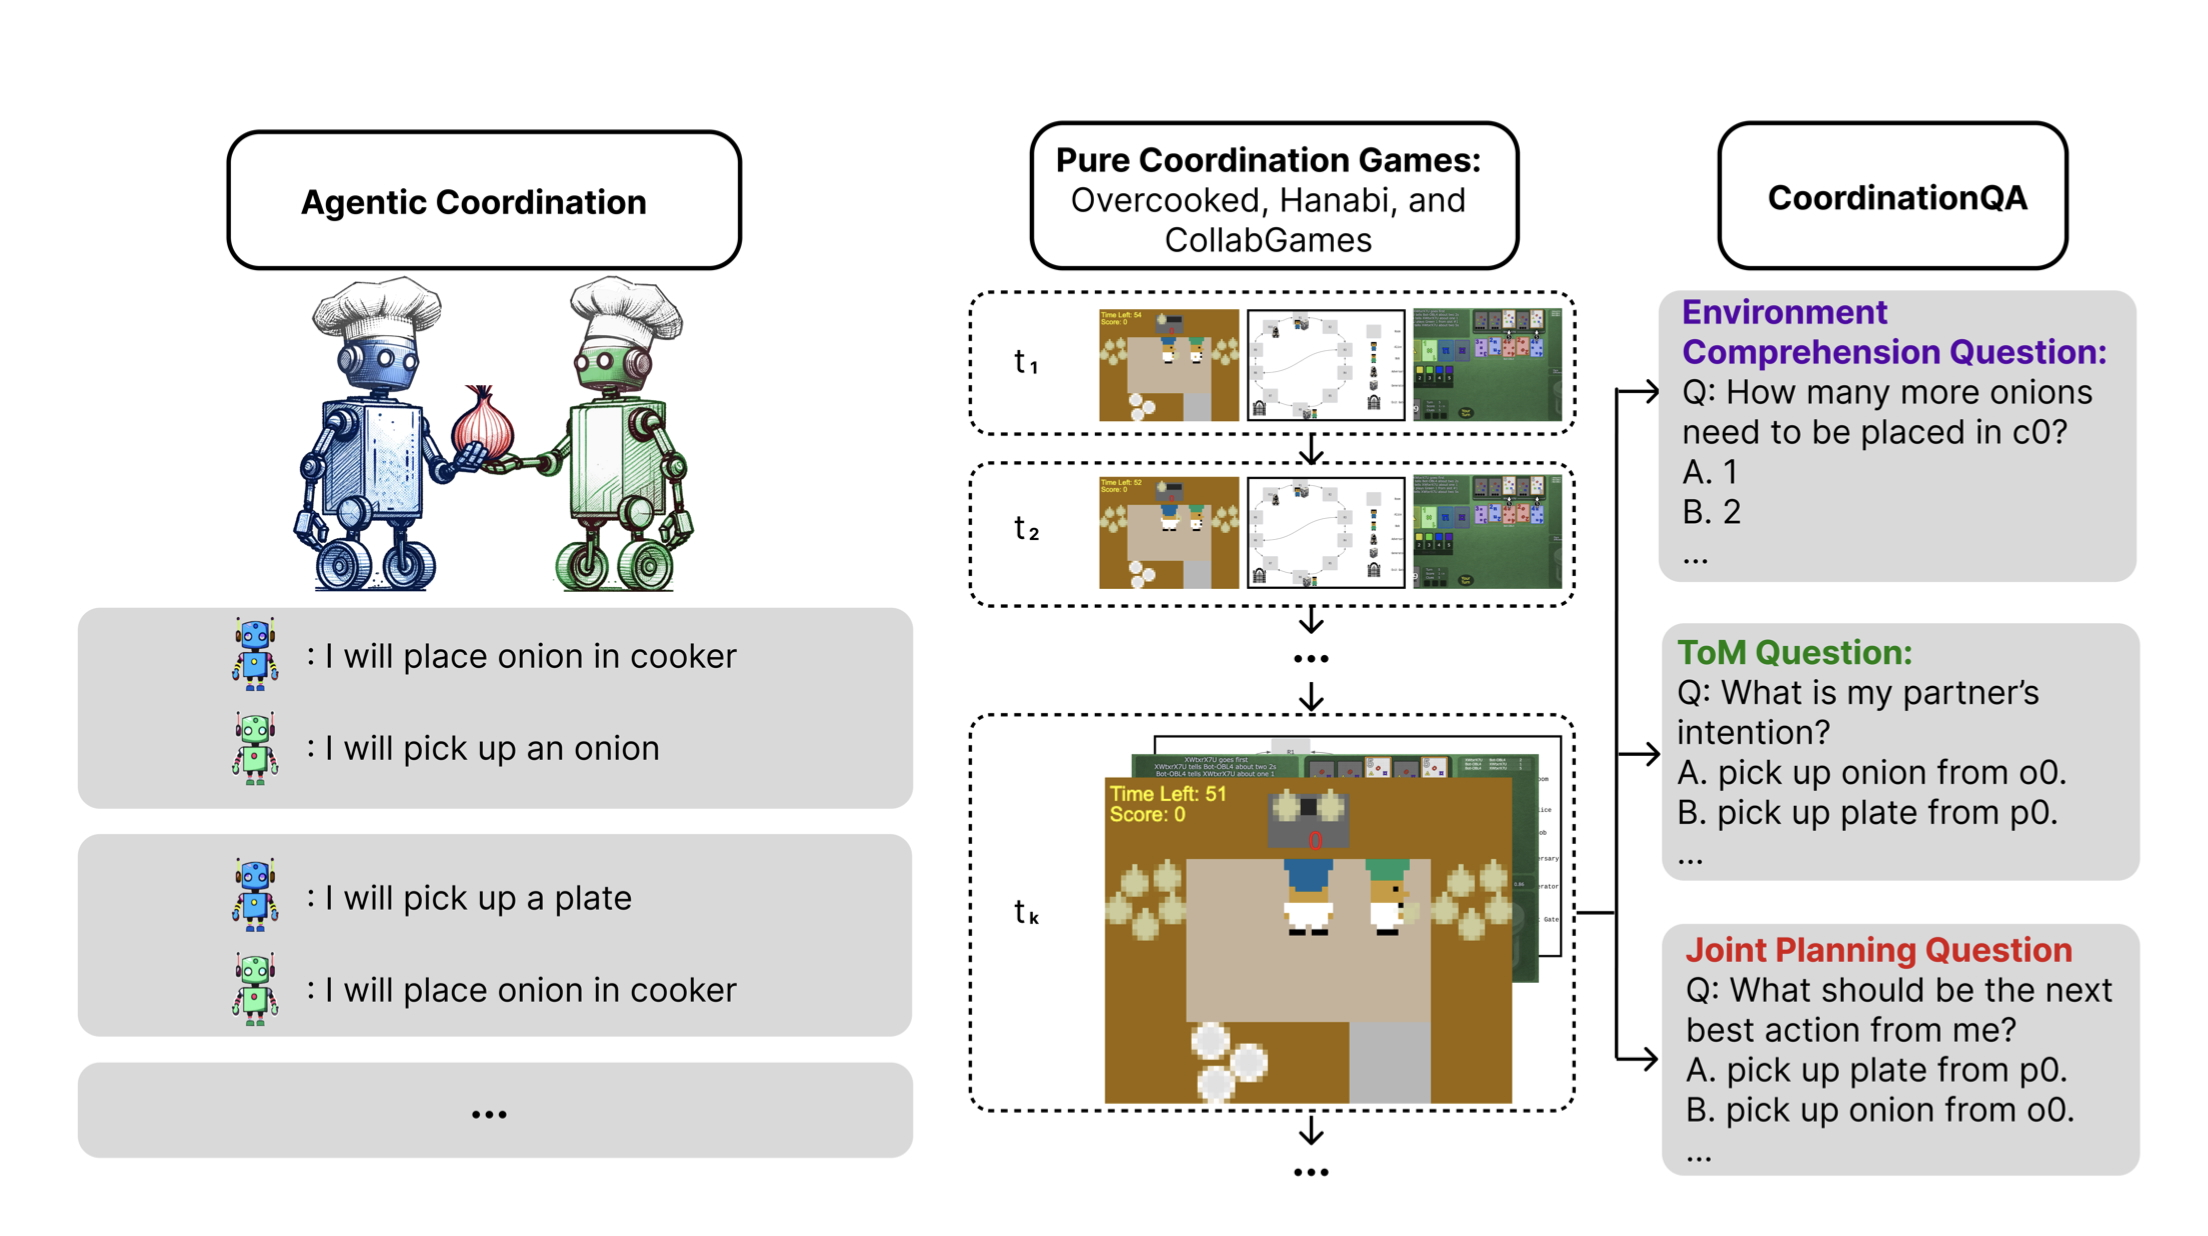
\includegraphics[width=2208pt]{figures/llmcoordinationbank.jpg}};
\fill[fill=white] (250,161) rectangle (723,244);
\node[anchor=center,inner sep=0pt,outer sep=0pt,align=center,text width=467pt,text=black,font={\fontsize{59.1429}{67.4229}\selectfont\sffamily\bfseries}] at (486.5,202.5) {智能体协调};
\fill[fill=white] (1040,133) rectangle (1510,261);
\node[anchor=center,inner sep=0pt,outer sep=0pt,align=center,text width=464pt,text=black,font={\fontsize{40.4143}{46.0723}\selectfont\sffamily}] at (1275,197) {\textbf{纯协调博弈：}\\Overcooked、Hanabi 与\\CollabGames};
\fill[fill={rgb,255:red,217;green,217;blue,217}] (305,632) rectangle (891,700);
\node[anchor=center,inner sep=0pt,outer sep=0pt,align=left,text width=580pt,text=black,font={\fontsize{44.85}{51.129}\selectfont\sffamily}] at (598,666) {：我会把洋葱放进烹饪锅。};
\fill[fill={rgb,255:red,217;green,217;blue,217}] (305,726) rectangle (891,791);
\node[anchor=center,inner sep=0pt,outer sep=0pt,align=left,text width=580pt,text=black,font={\fontsize{44.85}{51.129}\selectfont\sffamily}] at (598,758.5) {：我会取一个洋葱。};
\fill[fill={rgb,255:red,217;green,217;blue,217}] (305,877) rectangle (891,939);
\node[anchor=center,inner sep=0pt,outer sep=0pt,align=left,text width=580pt,text=black,font={\fontsize{44.85}{51.129}\selectfont\sffamily}] at (598,908) {：我会取一个盘子。};
\fill[fill={rgb,255:red,217;green,217;blue,217}] (305,972) rectangle (891,1031);
\node[anchor=center,inner sep=0pt,outer sep=0pt,align=left,text width=580pt,text=black,font={\fontsize{44.85}{51.129}\selectfont\sffamily}] at (598,1001.5) {：我会把洋葱放进烹饪锅。};
\fill[fill={rgb,255:red,217;green,217;blue,217}] (1676,295) rectangle (2125,574);
\node[anchor=north west,inner sep=0pt,outer sep=0pt,align=left,text width=429pt,text={rgb,255:red,107;green,0;blue,184},font={\fontsize{40.9071}{46.2251}\selectfont\sffamily}] at (1681,306) {\textbf{环境理解问题：}};
\node[anchor=north west,inner sep=0pt,outer sep=0pt,align=left,text width=429pt,text=black,font={\fontsize{38.4429}{43.4404}\selectfont\sffamily}] at (1681,355) {问：c0 还需放几个洋葱？\\A. 1\\B. 2\\……};
\fill[fill={rgb,255:red,217;green,217;blue,217}] (1675,634) rectangle (2124,869);
\node[anchor=north west,inner sep=0pt,outer sep=0pt,align=left,text width=429pt,text={rgb,255:red,17;green,132;blue,8},font={\fontsize{40.9071}{46.2251}\selectfont\sffamily}] at (1679,638) {\textbf{心智理论问题：}};
\node[anchor=north west,inner sep=0pt,outer sep=0pt,align=left,text width=429pt,text=black,font={\fontsize{38.4429}{43.4404}\selectfont\sffamily}] at (1679,686) {问：同伴打算做什么？\\A. 从 o0 取洋葱。\\B. 从 p0 取盘子。\\……};
\fill[fill={rgb,255:red,217;green,217;blue,217}] (1678,930) rectangle (2128,1165);
\node[anchor=north west,inner sep=0pt,outer sep=0pt,align=left,text width=432pt,text={rgb,255:red,223;green,24;blue,24},font={\fontsize{40.9071}{46.2251}\selectfont\sffamily}] at (1680,941) {\textbf{联合规划问题：}};
\node[anchor=north west,inner sep=0pt,outer sep=0pt,align=left,text width=432pt,text=black,font={\fontsize{38.4429}{43.4404}\selectfont\sffamily}] at (1680,990) {问：我的最佳下一步？\\A. 从 p0 取盘子。\\B. 从 o0 取洋葱。\\……};
\pgfresetboundingbox
\path[use as bounding box] (0,0) rectangle (2208,1236);
\end{tikzpicture}}
\endgroup

    \caption{LLM Coordination Benchmark 的示意图 \citep{agashe2025llm}。它采用两类测量评估智能体协调：一类是在纯协调博弈中的行为，智能体必须合作才能使收益最大化（中）；另一类是关于这些博弈的详细问题（右）。}\label{fig:agashe}
  \end{center}
\end{figure}

纯合作博弈的关键特征是，智能体必须完全相互合作，不存在竞争激励。相比之下，在囚徒困境等竞争情境中，或在 MAgIC 等基准测试中的混合动机博弈中，智能体的个体收益与集体收益之间存在真实的张力。在这类博弈中，如果大语言模型未能合作，其原因并不明确。智能体可能不善于协调，\textit{也可能}是在策略性地考虑个体收益。在纯合作博弈中，背叛从来没有理由，因此任何合作失败都确实体现了协调能力的不足。

\subsection{单一情境平台中的策略交互}
基准测试汇总了许多小型博弈的表现。另一条互补的研究路线则构建单一情境，深入研究智能体的行为。

Alympics \citep{mao2023alympics} 提供了一个受控试验场，用于模拟大语言模型驱动的智能体之间的策略交互。其中一个例子是多轮水资源分配挑战：必须随着时间推移分配稀缺的生存资源，见图~\ref{fig:water}。
\begin{figure}
  \begin{center}
    \begingroup
\linespread{1}\selectfont
\resizebox{\linewidth}{!}{%
\begin{tikzpicture}[x=1pt,y=-1pt]
\node[anchor=north west,inner sep=0pt,outer sep=0pt] at (0,0) {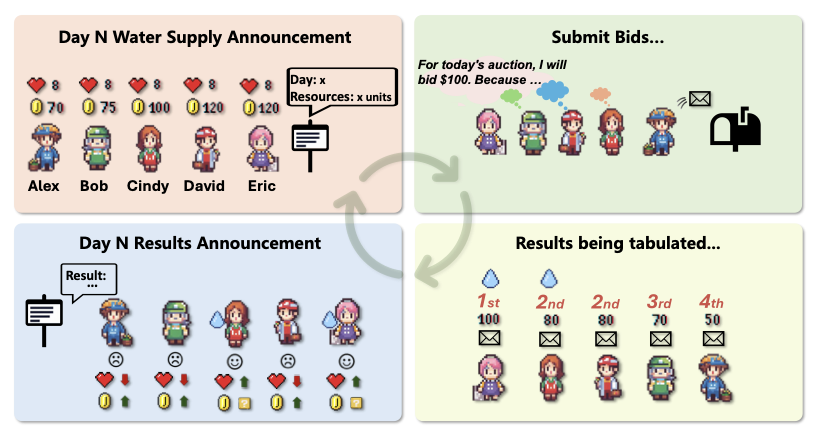
\includegraphics[width=822pt]{figures/water.png}};
\fill[fill={rgb,255:red,250;green,226;blue,215}] (42,25) rectangle (382,51);
\node[anchor=center,inner sep=0pt,outer sep=0pt,align=center,text width=334pt,text=black,font={\fontsize{19.0821}{21.7536}\selectfont\sffamily\bfseries}] at (212,38) {第 N 日供水公告};
\fill[fill={rgb,255:red,226;green,239;blue,215}] (530,25) rectangle (702,51);
\node[anchor=center,inner sep=0pt,outer sep=0pt,align=center,text width=166pt,text=black,font={\fontsize{18.8987}{21.5445}\selectfont\sffamily\bfseries}] at (616,38) {提交出价……};
\fill[fill={rgb,255:red,220;green,233;blue,247}] (68,229) rectangle (360,256);
\node[anchor=center,inner sep=0pt,outer sep=0pt,align=center,text width=286pt,text=black,font={\fontsize{18.7152}{21.3353}\selectfont\sffamily\bfseries}] at (214,242.5) {第 N 日结果公告};
\fill[fill={rgb,255:red,247;green,251;blue,220}] (485,229) rectangle (770,256);
\node[anchor=center,inner sep=0pt,outer sep=0pt,align=center,text width=279pt,text=black,font={\fontsize{18.7152}{21.3353}\selectfont\sffamily\bfseries}] at (627.5,242.5) {正在统计结果……};
\fill[fill={rgb,255:red,250;green,226;blue,215}] (291,71) rectangle (394,103);
\node[anchor=center,inner sep=0pt,outer sep=0pt,align=left,text width=97pt,text=black,font={\fontsize{12.1098}{13.8052}\selectfont\sffamily\bfseries}] at (342.5,87) {日期：x\\资源：x 单位};
\fill[fill={rgb,255:red,226;green,239;blue,215}] (417,54) rectangle (610,85);
\node[anchor=center,inner sep=0pt,outer sep=0pt,align=left,text width=187pt,text=black,font={\fontsize{13.2107}{15.0602}\selectfont\sffamily\bfseries}] at (513.5,69.5) {本日拍卖，我出价\$100，\\因为……};
\fill[fill={rgb,255:red,220;green,233;blue,247}] (65,269) rectangle (108,291);
\node[anchor=center,inner sep=0pt,outer sep=0pt,align=center,text width=37pt,text=black,font={\fontsize{10.4585}{11.9227}\selectfont\sffamily\bfseries}] at (86.5,280) {结果：\\……};
\fill[fill={rgb,255:red,247;green,251;blue,220}] (474,292) rectangle (527,312);
\node[anchor=center,inner sep=0pt,outer sep=0pt,align=center,text width=47pt,text={rgb,255:red,238;green,72;blue,64},font={\fontsize{11.9263}{13.596}\selectfont\sffamily\bfseries}] at (500.5,302) {第1名};
\fill[fill={rgb,255:red,247;green,251;blue,220}] (535,292) rectangle (588,312);
\node[anchor=center,inner sep=0pt,outer sep=0pt,align=center,text width=47pt,text={rgb,255:red,238;green,72;blue,64},font={\fontsize{11.9263}{13.596}\selectfont\sffamily\bfseries}] at (561.5,302) {第2名};
\fill[fill={rgb,255:red,247;green,251;blue,220}] (591,292) rectangle (644,312);
\node[anchor=center,inner sep=0pt,outer sep=0pt,align=center,text width=47pt,text={rgb,255:red,238;green,72;blue,64},font={\fontsize{11.9263}{13.596}\selectfont\sffamily\bfseries}] at (617.5,302) {第2名};
\fill[fill={rgb,255:red,247;green,251;blue,220}] (648,292) rectangle (701,312);
\node[anchor=center,inner sep=0pt,outer sep=0pt,align=center,text width=47pt,text={rgb,255:red,238;green,72;blue,64},font={\fontsize{11.9263}{13.596}\selectfont\sffamily\bfseries}] at (674.5,302) {第3名};
\fill[fill={rgb,255:red,247;green,251;blue,220}] (702,292) rectangle (755,312);
\node[anchor=center,inner sep=0pt,outer sep=0pt,align=center,text width=47pt,text={rgb,255:red,238;green,72;blue,64},font={\fontsize{11.9263}{13.596}\selectfont\sffamily\bfseries}] at (728.5,302) {第4名};
\pgfresetboundingbox
\path[use as bounding box] (0,0) rectangle (822,444);
\end{tikzpicture}}
\endgroup

    \caption{Alympics 水资源分配挑战游戏 \citep{mao2023alympics}}\label{fig:water}
  \end{center}
\end{figure}

AucArena \citep{chen2023put} 使用 LLaMa 2.13b、Mistral 7b、Mixtral 8x7b、Gemini 1.0 和 GPT 3.5/4.0 模拟拍卖。研究发现，GPT-4 等能力最强的大语言模型具有参与拍卖所需的技能，例如预算管理与目标专注；不过，即使这一模型的表现也存在波动，作者指出，其表现仍有很大的提升空间。

\subsection{小结}
无论是跨博弈的基准测试，还是单一情境平台，协调始终都是大语言模型智能体的薄弱环节。较强的大语言模型在 MAgIC 的理性与判断指标上得分较高，在 AucArena 中能够合理管理预算，在由环境驱动的合作任务中能够达到经过训练的强化学习智能体的水平。然而，当成功需要推理同伴的信念与意图时，除了最强且得到最充分支架支持的模型之外，其他模型都会失败。

换言之，模型无法始终如一地将心智理论推理与自身行为\emph{整合}起来。在第~\ref{chap:behavior}~章中，这类失败被称为知行鸿沟（knowing-doing gap）或字面—功能鸿沟（literal-functional gap）：GPT-4 在被要求预测巴赫或斯特拉文斯基博弈（Bach or Stravinsky）中的交替模式时，能够准确回答，却无法在实际对局中执行这一模式。然而，本节回顾的多智能体研究使这一诊断变得更复杂。在 LLM Coordination Benchmark 的问答部分，联合规划问题所提出的，恰好就是智能体在游戏每一步面对的决策。模型在这些问题上的表现最差，而在心智理论问题上的表现也好不了多少。在各项博弈中，问答得分与智能体表现呈正相关。也就是说，在这里，知与行同步变化：模型行动表现不佳时，即便直接向它们提出行动问题，其推理表现也同样不佳。因此，对于纯协调任务，缺陷在于采纳同伴的视角（心智理论）与联合规划本身，而不是在于将推理转化为行动。

在另一个层面，知行鸿沟又出现了。在 Hanabi 中，只有加入明确的心智理论推理与自我验证步骤作为支架，GPT-4-turbo 才能达到尚可的表现。缺少这些步骤时，它在每次 Hanabi 测试中都会犯下致命错误。换言之，它最初的行动是错误的，但当提示要求它检查推理与验证步骤时，它就能识别并纠正这些错误。类似的表现提升也见于 MAgIC 中的概率图建模，以及第~\ref{chap:behavior}~章策略行为研究中的社会思维链（Social Chain-of-Thought）。\emph{大语言模型无法推理他人}与\emph{大语言模型不会自发运用这种推理}之间的界限，显然十分微妙；将结构化推理与验证步骤嵌入智能体，能够使后一种潜在能力显现出来。

下一节考察对同一问题的另一种互补回应：不提升智能体的推理能力，而是通过分配角色来组织交互本身。

\section{基于角色的任务求解与团队合作}\label{sec:roletask}
上一节中的智能体是地位对称的同伴，协调必须从其自身的策略推理中产生，成效却很有限。本节讨论的研究通过交互协议，以及具有不同目标的角色分配，将协调纳入系统设计之中。

按照第~\ref{fivedimensions}~节定义的五个维度，这些研究改变了\emph{策略}与\emph{结构}，同时保持总体交互类型为合作。我们将依次讨论从简单到复杂的结构：互补配对、多方辩论、团队，以及压力之下的社会角色扮演。

\subsection{互补配对}
大语言模型可以成对执行任务，并被赋予互补角色，例如创作者—批评者或管理者—工作者。在这些配对方案中，每个大语言模型智能体都具有不同的角色与目标，并通过通信共同求解任务。

在 CAMEL 框架（Communicative Agents for ``Mind'' Exploration，即用于“心智”探索的交流智能体）\citep{li2023camel} 中，两个大语言模型各自承担预先定义的角色，共同朝某个目标工作，例如完成编程任务（见图~\ref{fig:camel}）。它们通过合作共同推动对话，无须人类持续提供明确提示。CAMEL 使用初始提示（inception prompting）与角色描述，使智能体保持角色，并朝目标协作。提示要求智能体在对话过程中，将复杂问题分解为易于处理的步骤。在每一步交互中，大语言模型智能体实际上都在生成自己的推理阶段训练数据，使人类能够检查其认知过程，同时提高自主执行任务的表现。

\begin{figure}[!htb]
  \begin{center}
    \begingroup
\linespread{1}\selectfont
\resizebox{\linewidth}{!}{%
\begin{tikzpicture}[x=1pt,y=-1pt]
\node[anchor=north west,inner sep=0pt,outer sep=0pt] at (0,0) {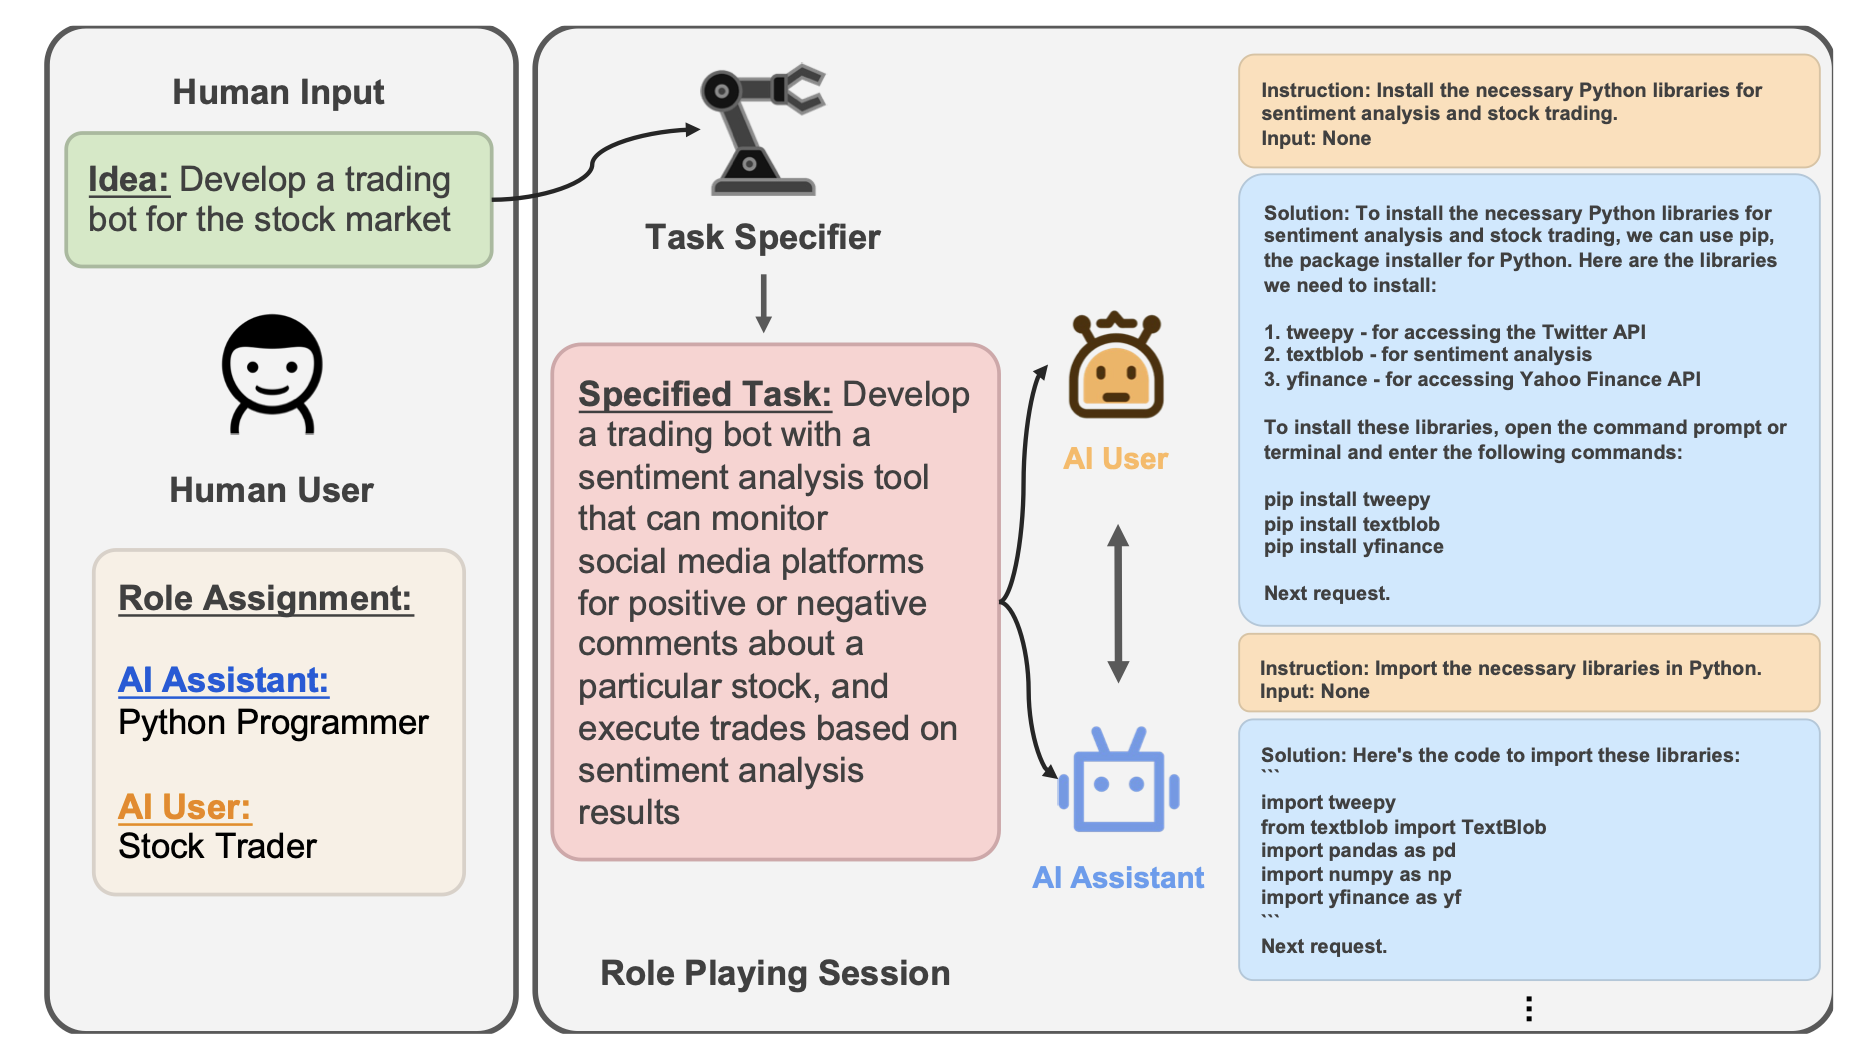
\includegraphics[width=1876pt]{figures/CAMEL.png}};
\fill[fill={rgb,255:red,243;green,243;blue,243}] (153,68) rectangle (418,118);
\node[anchor=center,inner sep=0pt,outer sep=0pt,align=center,text width=259pt,text=black,font={\fontsize{51.925}{59.1945}\selectfont\sffamily\bfseries}] at (285.5,93) {人类输入};
\fill[fill={rgb,255:red,213;green,231;blue,198}] (75,145) rectangle (482,255);
\node[anchor=center,inner sep=0pt,outer sep=0pt,align=center,text width=401pt,text=black,font={\fontsize{42.7125}{48.6922}\selectfont\sffamily}] at (278.5,200) {\textbf{构想：}开发一个\\股票市场交易机器人};
\fill[fill={rgb,255:red,243;green,243;blue,243}] (153,465) rectangle (423,516);
\node[anchor=center,inner sep=0pt,outer sep=0pt,align=center,text width=264pt,text=black,font={\fontsize{51.925}{59.1945}\selectfont\sffamily\bfseries}] at (288,490.5) {人类用户};
\fill[fill={rgb,255:red,248;green,239;blue,227}] (110,573) rectangle (446,626);
\node[anchor=center,inner sep=0pt,outer sep=0pt,align=center,text width=330pt,text=black,font={\fontsize{44.8062}{51.0791}\selectfont\sffamily\bfseries}] at (278,599.5) {角色分配：};
\fill[fill={rgb,255:red,248;green,239;blue,227}] (110,656) rectangle (447,700);
\node[anchor=center,inner sep=0pt,outer sep=0pt,align=left,text width=331pt,text={rgb,255:red,9;green,85;blue,230},font={\fontsize{44.8062}{51.0791}\selectfont\sffamily\bfseries}] at (278.5,678) {AI 助手：};
\fill[fill={rgb,255:red,248;green,239;blue,227}] (110,704) rectangle (447,754);
\node[anchor=center,inner sep=0pt,outer sep=0pt,align=left,text width=331pt,text=black,font={\fontsize{44.8062}{51.0791}\selectfont\sffamily}] at (278.5,729) {Python 程序员};
\fill[fill={rgb,255:red,248;green,239;blue,227}] (110,781) rectangle (447,824);
\node[anchor=center,inner sep=0pt,outer sep=0pt,align=left,text width=331pt,text={rgb,255:red,233;green,139;blue,0},font={\fontsize{44.8062}{51.0791}\selectfont\sffamily\bfseries}] at (278.5,802.5) {AI 用户：};
\fill[fill={rgb,255:red,248;green,239;blue,227}] (110,828) rectangle (447,876);
\node[anchor=center,inner sep=0pt,outer sep=0pt,align=left,text width=331pt,text=black,font={\fontsize{44.8062}{51.0791}\selectfont\sffamily}] at (278.5,852) {股票交易员};
\fill[fill={rgb,255:red,243;green,243;blue,243}] (630,211) rectangle (907,264);
\node[anchor=center,inner sep=0pt,outer sep=0pt,align=center,text width=271pt,text=black,font={\fontsize{51.5063}{58.7171}\selectfont\sffamily\bfseries}] at (768.5,237.5) {任务细化器};
\fill[fill={rgb,255:red,250;green,209;blue,207}] (573,365) rectangle (978,838);
\node[anchor=north west,inner sep=0pt,outer sep=0pt,align=left,text width=393pt,text=black,font={\fontsize{43.1313}{48.7383}\selectfont\sffamily}] at (578,370) {\textbf{具体任务：}开发一个带有情绪分析工具的交易机器人，监测社交媒体平台上关于某只股票的正面或负面评论，并根据情绪分析结果执行交易。};
\fill[fill={rgb,255:red,243;green,243;blue,243}] (1033,439) rectangle (1212,479);
\node[anchor=center,inner sep=0pt,outer sep=0pt,align=center,text width=173pt,text={rgb,255:red,252;green,179;blue,79},font={\fontsize{43.55}{49.647}\selectfont\sffamily\bfseries}] at (1122.5,459) {AI 用户};
\fill[fill={rgb,255:red,243;green,243;blue,243}] (1024,864) rectangle (1217,911);
\node[anchor=center,inner sep=0pt,outer sep=0pt,align=center,text width=187pt,text={rgb,255:red,96;green,153;blue,239},font={\fontsize{43.55}{49.647}\selectfont\sffamily\bfseries}] at (1120.5,887.5) {AI 助手};
\fill[fill={rgb,255:red,243;green,243;blue,243}] (590,948) rectangle (985,1002);
\node[anchor=center,inner sep=0pt,outer sep=0pt,align=center,text width=389pt,text=black,font={\fontsize{49.4125}{56.3303}\selectfont\sffamily\bfseries}] at (787.5,975) {角色扮演会话};
\fill[fill={rgb,255:red,243;green,243;blue,243}] (531,1008) rectangle (1840,1260);
\draw[draw=black!65,line width=5pt,rounded corners=40pt] (534,28) rectangle (1834,1255);
\fill[fill={rgb,255:red,243;green,243;blue,243}] (1236,51) rectangle (1825,1234);
\draw[fill={rgb,255:red,255;green,224;blue,183},draw={rgb,255:red,214;green,192;blue,159},line width=2pt,rounded corners=18pt] (1239,55) rectangle (1820,183);
\node[anchor=north west,inner sep=0pt,outer sep=0pt,align=left,text width=536pt,text=black,font={\fontsize{34.7563}{39.2746}\selectfont\sffamily}] at (1260,70) {\textbf{指令：}安装情绪分析与股票交易所需的 Python 库。\\\textbf{输入：}无};
\draw[fill={rgb,255:red,202;green,231;blue,250},draw={rgb,255:red,174;green,203;blue,220},line width=2pt,rounded corners=18pt] (1239,192) rectangle (1820,716);
\node[anchor=north west,inner sep=0pt,outer sep=0pt,align=left,text width=536pt,text=black,font={\fontsize{32.6625}{36.9086}\selectfont\sffamily}] at (1260,208) {\textbf{解决方案：}可用 Python 的软件包安装器 pip，安装情绪分析和股票交易所需的库。需要安装：\\1. tweepy：访问 Twitter API\\2. textblob：情绪分析\\3. yfinance：访问 Yahoo Finance API\\[0.2em]请打开命令提示符或终端，输入以下命令：\\\texttt{pip install tweepy}\\\texttt{pip install textblob}\\\texttt{pip install yfinance}\\[0.2em]下一项请求。};
\draw[fill={rgb,255:red,255;green,224;blue,183},draw={rgb,255:red,214;green,192;blue,159},line width=2pt,rounded corners=18pt] (1239,725) rectangle (1820,818);
\node[anchor=north west,inner sep=0pt,outer sep=0pt,align=left,text width=536pt,text=black,font={\fontsize{34.7563}{39.2746}\selectfont\sffamily}] at (1260,739) {\textbf{指令：}在 Python 中导入所需的库。\\\textbf{输入：}无};
\draw[fill={rgb,255:red,202;green,231;blue,250},draw={rgb,255:red,174;green,203;blue,220},line width=2pt,rounded corners=18pt] (1239,827) rectangle (1820,1215);
\node[anchor=north west,inner sep=0pt,outer sep=0pt,align=left,text width=536pt,text=black,font={\fontsize{33.5}{37.855}\selectfont\sffamily}] at (1260,842) {\textbf{解决方案：}以下代码用于导入这些库：\\\texttt{```}\\\texttt{import tweepy}\\\texttt{from textblob import TextBlob}\\\texttt{import pandas as pd}\\\texttt{import numpy as np}\\\texttt{import yfinance as yf}\\\texttt{```}\\下一项请求。};
\node[anchor=north west,inner sep=0pt,outer sep=0pt,align=left,text width=50pt,text=black,font={\fontsize{41.875}{47.3187}\selectfont\sffamily}] at (1510,1223) {$\vdots$};
\pgfresetboundingbox
\path[use as bounding box] (0,0) rectangle (1876,1270);
\end{tikzpicture}}
\endgroup

    \caption{CAMEL 中的角色扮演 \citep{li2023camel}}\label{fig:camel}
  \end{center}
\end{figure}

其他研究在自我反思情境中，将一个充当创作者（或生成器）的大语言模型，与另一个充当裁判（或批评者）的大语言模型配对。这样，一个智能体发挥大语言模型的生成能力，另一个则督促其遵守规则或质量准则。Constitutional AI \citep{bai2022constitutional} 使用一个大语言模型，依据一组伦理或质量准则，评议另一个大语言模型的回答，并提出修改建议。作者表明，这种双智能体反馈能够产出经过改进、且符合预期原则的最终结果。

第三种配对交互遵循人类辅导的模式：教师—学习者或专家—新手。第~\ref{sec:distillation}~章在蒸馏的背景下讨论了这一结构的多个例子。

这三种配对都利用了同一个思路：一个智能体的监督可以纠正另一个智能体的错误，使联合表现比任一智能体独立工作时更加稳健。

\subsection{辩论与讨论}
除配对之外，基于角色的交互还有一个突出例子：利用大语言模型之间的辩论与讨论，改善推理和任务表现。

\citet{du2024debate} 表明，当多个大语言模型实例先提出答案，再通过多轮辩论相互评议推理时，它们能够达成更准确的共识答案，事实正确性也更高。该方法以 Minsky 的心智社会（society of minds）\citep{minsky1988society} 为概念描述，在数学文字题与事实问答等任务中，显著减少了推理错误与幻觉。

\citet{liang-etal-2024-encouraging} 提出了一种多智能体辩论（multi-agent debate，MAD）方案：两个大语言模型智能体持相反立场，例如进行一报还一报（tit-for-tat）式谈判（见第~\ref{sec:strategic}~节），第三个智能体则担任裁判。裁判的角色是引导讨论走向最终解决方案。结构化辩论鼓励发散思维，并能使经过 MAD 增强的较弱模型（如 GPT-3.5）在具有挑战性的基准测试中，超过未采用 MAD 的较强模型（如 GPT-4）。作者讨论了他们的 MAD 方案如何克服在模型中加入自我反思步骤作为支架时的一个已知问题。自我反思可能引发所谓的\emph{思维退化（degeneration of thought）}：一旦模型对某个求解方向产生信心，即使方向错误，自我反思也可能进一步强化这种信心。在 MAD 辩论方案中，另一个智能体可以推动模型转向不同方向，从而避免思维退化。

ChatEval 将这种辩论模式用于文本评估 \citep{chan2023chateval}。作者注意到，多位标注者协作可以改善人类文本评估的质量，于是构建了一支多智能体评审团队，其中包含辩论智能体、多样的角色设定和不同的通信策略（见图~\ref{fig:chateval}），超越了单智能体提示策略。

\begin{figure}
  \begin{center}
    \begingroup
\linespread{1}\selectfont
\resizebox{\linewidth}{!}{%
\begin{tikzpicture}[x=1pt,y=-1pt]
\node[anchor=north west,inner sep=0pt,outer sep=0pt] at (0,0) {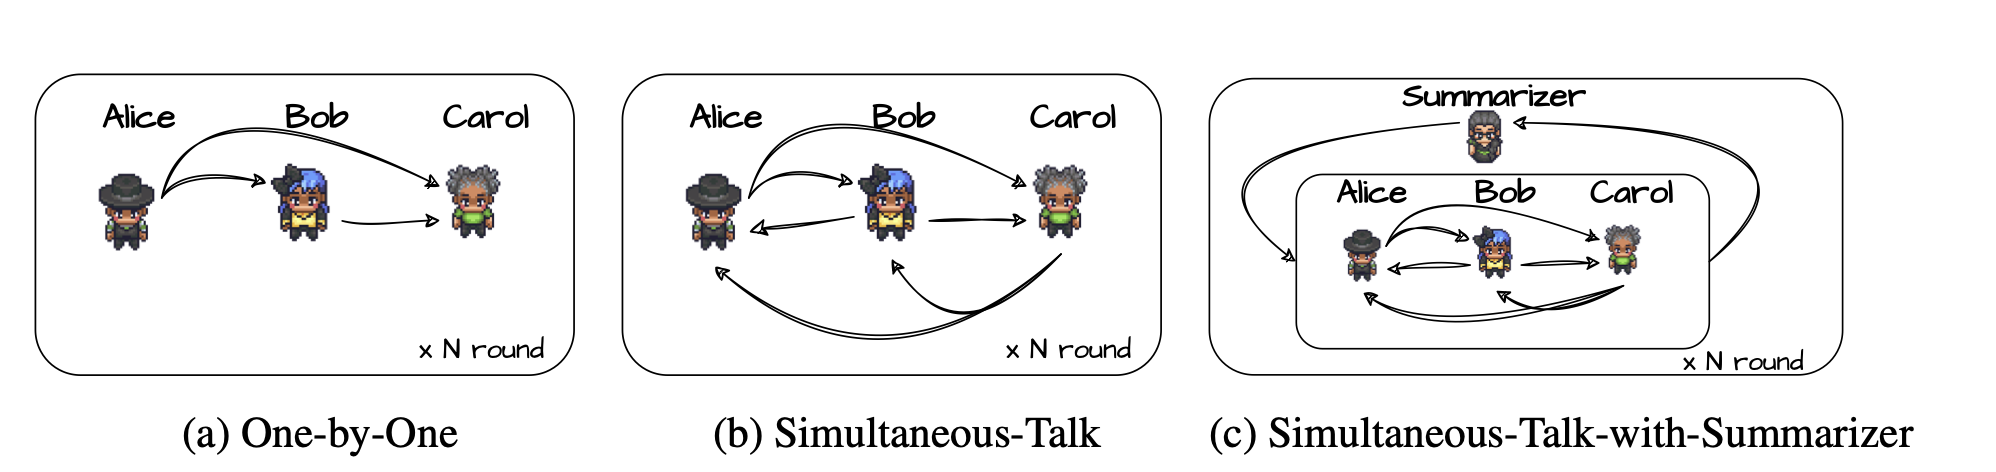
\includegraphics[width=1996pt]{figures/chateval.png}};
\fill[fill=white] (1392,81) rectangle (1616,111);
\fill[fill=white] (1270,87) rectangle (1445,126);
\node[anchor=center,inner sep=0pt,outer sep=0pt,align=center,text width=169pt,text=black,font={\fontsize{33.4152}{38.0933}\selectfont\sffamily\bfseries}] at (1357.5,106.5) {总结器};
\fill[fill=white] (1678,349) rectangle (1831,372);
\fill[fill=white] (380,334) rectangle (554,367);
\node[anchor=center,inner sep=0pt,outer sep=0pt,align=center,text width=168pt,text=black,font={\fontsize{36.0884}{41.1408}\selectfont\sffamily}] at (467,350.5) {重复 $N$ 轮};
\fill[fill=white] (965,334) rectangle (1139,367);
\node[anchor=center,inner sep=0pt,outer sep=0pt,align=center,text width=168pt,text=black,font={\fontsize{36.0884}{41.1408}\selectfont\sffamily}] at (1052,350.5) {重复 $N$ 轮};
\fill[fill=white] (1718,267) rectangle (1827,333);
\node[anchor=center,inner sep=0pt,outer sep=0pt,align=center,text width=103pt,text=black,font={\fontsize{31.1875}{35.5537}\selectfont\sffamily}] at (1772.5,300) {重复\\$N$ 轮};
\draw[draw=black,line width=1.7pt] (1797,375) .. controls (1822,375) and (1843,355) .. (1843,330);
\fill[fill=white] (143,404) rectangle (568,470);
\node[anchor=center,inner sep=0pt,outer sep=0pt,align=center,text width=419pt,text=black,font={\fontsize{46.7812}{53.3306}\selectfont\sffamily}] at (355.5,437) {(a) 逐一发言};
\fill[fill=white] (690,404) rectangle (1175,470);
\node[anchor=center,inner sep=0pt,outer sep=0pt,align=center,text width=479pt,text=black,font={\fontsize{46.7812}{53.3306}\selectfont\sffamily}] at (932.5,437) {(b) 同时发言};
\fill[fill=white] (1200,404) rectangle (1960,470);
\node[anchor=center,inner sep=0pt,outer sep=0pt,align=center,text width=754pt,text=black,font={\fontsize{46.7812}{53.3306}\selectfont\sffamily}] at (1580,437) {(c) 带总结器的同时发言};
\pgfresetboundingbox
\path[use as bounding box] (0,0) rectangle (1996,472);
\end{tikzpicture}}
\endgroup

    \caption{ChatEval 中三种不同的通信策略 \citep{chan2023chateval}}\label{fig:chateval}
  \end{center}
\end{figure}

另一种同样受 Minsky 心智社会启发的方法是 ReConcile。这一多智能体框架被设计为由多样化大语言模型智能体参加的圆桌会议 \citep{chen2023reconcile}。框架通过多轮讨论增强大语言模型智能体之间的协作推理。智能体必须尝试说服彼此，以改进各自的答案。七项基准测试上的实验表明，置信度加权投票机制能够显著改善大语言模型的推理。此外，作者发现，多样性，即使用不同的底层模型，对表现至关重要。

MindStorms 引入了一种基于大语言模型的实现 \citep{zhuge2023mindstorms}，以 CAMEL 框架 \citep{li2023camel} 为基础。该研究报告了大量实验，最多使用 129 个智能体解决常见人工智能问题，包括视觉问答、图像描述、文本生成图像、三维生成、第一人称检索、具身人工智能，以及一般的基于语言的任务求解。作者发现，在特定应用中，由更多成员参与的头脑风暴优于成员较少的头脑风暴，持续时间更长的头脑风暴也优于较短的头脑风暴。

\subsection{基于角色的软件团队}
基于角色的协作有一个有趣的应用：软件开发。完全由大语言模型智能体组成的模拟团队负责开发软件。

大语言模型自动编程一直受到若干问题的困扰，例如逻辑不一致，以及沿整个开发流程级联传播的幻觉。MetaGPT \citep{hong2024metagpt} 借鉴了在人类软件团队中已被证明有效的工作流程。该框架将标准操作协议（Standard Operation Protocols，SOP）转换为提示序列，并为智能体分配软件公司中的角色：产品经理、架构师、工程师、质量保证测试人员。这样，智能体沿着一条流水线传递结构化的中间产物。产品经理编写需求文档，架构师将其转化为设计，工程师负责编码。通过这种方式，复杂任务被分解为易于处理的子任务，智能体能够逐步验证过程，从而显著减少错误。

类似地，\citet{qian-etal-2024-chatdev} 提出了虚拟软件公司 ChatDev，智能体在其中协作完成开发流程的各个阶段：设计、编码与测试。协作按照\emph{对话链（chat chain）}组织：每个阶段都被分解为指导者与助手智能体之间的简短对话（见图~\ref{fig:chatdev2}）。采用一种要求智能体在回答前询问更多细节的通信协议，可以实现作者所说的\emph{去幻觉（dehallucination）}，提高每一步的可靠性。该框架展示了结构化自然语言通信如何促进多智能体协作。

\begin{figure}
  \begin{center}
    \begingroup
\linespread{1}\selectfont
\resizebox{\linewidth}{!}{%
\begin{tikzpicture}[x=1pt,y=-1pt]
\node[anchor=north west,inner sep=0pt,outer sep=0pt] at (0,0) {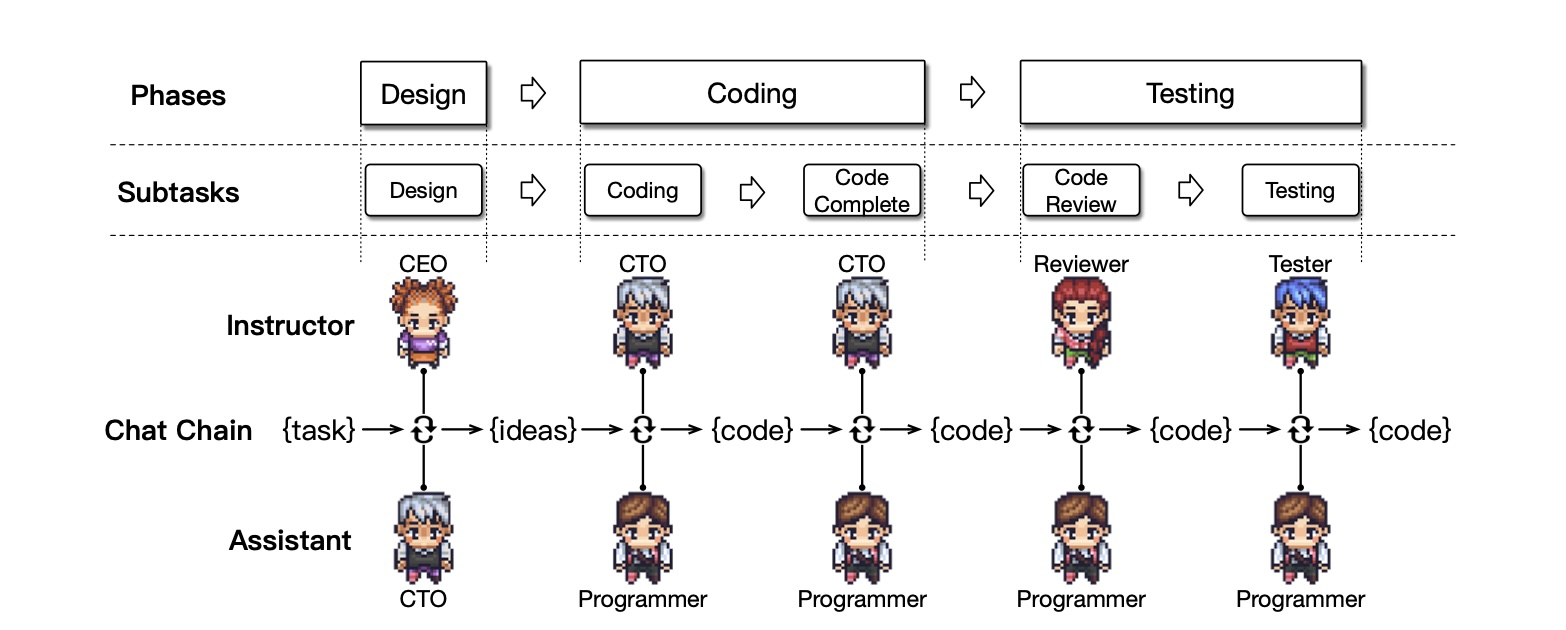
\includegraphics[width=1566pt]{figures/chatdev2.jpg}};
\draw[fill=white,draw={rgb,255:red,37;green,37;blue,37},line width=1.5pt,rounded corners=4pt] (803,163) rectangle (921,217);
\draw[fill=white,draw={rgb,255:red,37;green,37;blue,37},line width=1.5pt,rounded corners=4pt] (1023,163) rectangle (1141,217);
\fill[fill=white] (125,78) rectangle (234,112);
\node[anchor=center,inner sep=0pt,outer sep=0pt,align=center,text width=103pt,text=black,font={\fontsize{36.004}{41.0446}\selectfont\sffamily\bfseries}] at (179.5,95) {阶段};
\fill[fill=white] (375,76) rectangle (477,111);
\node[anchor=center,inner sep=0pt,outer sep=0pt,align=center,text width=96pt,text=black,font={\fontsize{36.004}{41.0446}\selectfont\sffamily}] at (426,93.5) {设计};
\fill[fill=white] (700,77) rectangle (818,111);
\node[anchor=center,inner sep=0pt,outer sep=0pt,align=center,text width=112pt,text=black,font={\fontsize{36.004}{41.0446}\selectfont\sffamily}] at (759,94) {编码};
\fill[fill=white] (1135,77) rectangle (1255,111);
\node[anchor=center,inner sep=0pt,outer sep=0pt,align=center,text width=114pt,text=black,font={\fontsize{36.004}{41.0446}\selectfont\sffamily}] at (1195,94) {测试};
\fill[fill=white] (113,176) rectangle (254,212);
\node[anchor=center,inner sep=0pt,outer sep=0pt,align=center,text width=135pt,text=black,font={\fontsize{36.004}{41.0446}\selectfont\sffamily\bfseries}] at (183.5,194) {子任务};
\fill[fill=white] (382,174) rectangle (474,211);
\node[anchor=center,inner sep=0pt,outer sep=0pt,align=center,text width=86pt,text=black,font={\fontsize{32.858}{37.4582}\selectfont\sffamily}] at (428,192.5) {设计};
\fill[fill=white] (593,174) rectangle (697,211);
\node[anchor=center,inner sep=0pt,outer sep=0pt,align=center,text width=98pt,text=black,font={\fontsize{32.858}{37.4582}\selectfont\sffamily}] at (645,192.5) {编码};
\fill[fill=white] (808,167) rectangle (918,213);
\node[anchor=center,inner sep=0pt,outer sep=0pt,align=center,text width=104pt,text=black,font={\fontsize{25.5174}{29.0898}\selectfont\sffamily}] at (863,190) {代码补全};
\fill[fill=white] (1028,167) rectangle (1137,213);
\node[anchor=center,inner sep=0pt,outer sep=0pt,align=center,text width=103pt,text=black,font={\fontsize{25.5174}{29.0898}\selectfont\sffamily}] at (1082.5,190) {代码评审};
\fill[fill=white] (1267,175) rectangle (1351,211);
\node[anchor=center,inner sep=0pt,outer sep=0pt,align=center,text width=78pt,text=black,font={\fontsize{32.858}{37.4582}\selectfont\sffamily}] at (1309,193) {测试};
\fill[fill=white] (219,310) rectangle (360,342);
\node[anchor=center,inner sep=0pt,outer sep=0pt,align=center,text width=135pt,text=black,font={\fontsize{35.6545}{40.6461}\selectfont\sffamily\bfseries}] at (289.5,326) {指导者};
\fill[fill=white] (100,412) rectangle (256,449);
\node[anchor=center,inner sep=0pt,outer sep=0pt,align=center,text width=150pt,text=black,font={\fontsize{35.6545}{40.6461}\selectfont\sffamily\bfseries}] at (178,430.5) {对话链};
\fill[fill=white] (224,527) rectangle (359,562);
\node[anchor=center,inner sep=0pt,outer sep=0pt,align=center,text width=129pt,text=black,font={\fontsize{35.6545}{40.6461}\selectfont\sffamily\bfseries}] at (291.5,544.5) {助手};
\fill[fill=white] (1024,250) rectangle (1142,276);
\node[anchor=center,inner sep=0pt,outer sep=0pt,align=center,text width=112pt,text=black,font={\fontsize{30.7607}{35.0672}\selectfont\sffamily}] at (1083,263) {评审者};
\fill[fill=white] (1250,250) rectangle (1355,276);
\node[anchor=center,inner sep=0pt,outer sep=0pt,align=center,text width=99pt,text=black,font={\fontsize{30.7607}{35.0672}\selectfont\sffamily}] at (1302.5,263) {测试者};
\fill[fill=white] (568,586) rectangle (719,617);
\node[anchor=center,inner sep=0pt,outer sep=0pt,align=center,text width=145pt,text=black,font={\fontsize{31.1103}{35.4657}\selectfont\sffamily}] at (643.5,601.5) {程序员};
\fill[fill=white] (789,586) rectangle (940,617);
\node[anchor=center,inner sep=0pt,outer sep=0pt,align=center,text width=145pt,text=black,font={\fontsize{31.1103}{35.4657}\selectfont\sffamily}] at (864.5,601.5) {程序员};
\fill[fill=white] (1008,586) rectangle (1159,617);
\node[anchor=center,inner sep=0pt,outer sep=0pt,align=center,text width=145pt,text=black,font={\fontsize{31.1103}{35.4657}\selectfont\sffamily}] at (1083.5,601.5) {程序员};
\fill[fill=white] (1228,586) rectangle (1379,617);
\node[anchor=center,inner sep=0pt,outer sep=0pt,align=center,text width=145pt,text=black,font={\fontsize{31.1103}{35.4657}\selectfont\sffamily}] at (1303.5,601.5) {程序员};
\pgfresetboundingbox
\path[use as bounding box] (0,0) rectangle (1566,630);
\end{tikzpicture}}
\endgroup

    \caption{ChatDev 中的链式工作流程 \citep{qian-etal-2024-chatdev}，以 ChatGPT-3.5 驱动的智能体之间的多轮双边通信为基础。}\label{fig:chatdev2}
  \end{center}
\end{figure}

MetaGPT 与 ChatDev 将特定的组织结构固定在系统中，而 AutoGen \citep{wu2024autogen} 则提供了一个灵活的编程框架，以可定制智能体之间的对话为基础，将大语言模型、工具和人类输入结合起来。它被设计为开放源代码平台，让开发者能够根据应用定义智能体与交互结构。实验表明，该框架在数学、编程、问答、娱乐等领域的任务中均有效。

\subsection{社会角色扮演}
上述系统分配角色是为了解决任务。最后一条研究路线则为了研究社会行为本身而分配角色：当大语言模型智能体被置于社会要求较高或存在冲突的情境中时，它们会如何行动？

\begin{figure}
  \begin{center}
    \begingroup
\linespread{1}\selectfont
\resizebox{\linewidth}{!}{%
\begin{tikzpicture}[x=1pt,y=-1pt]
\node[anchor=north west,inner sep=0pt,outer sep=0pt] at (0,0) {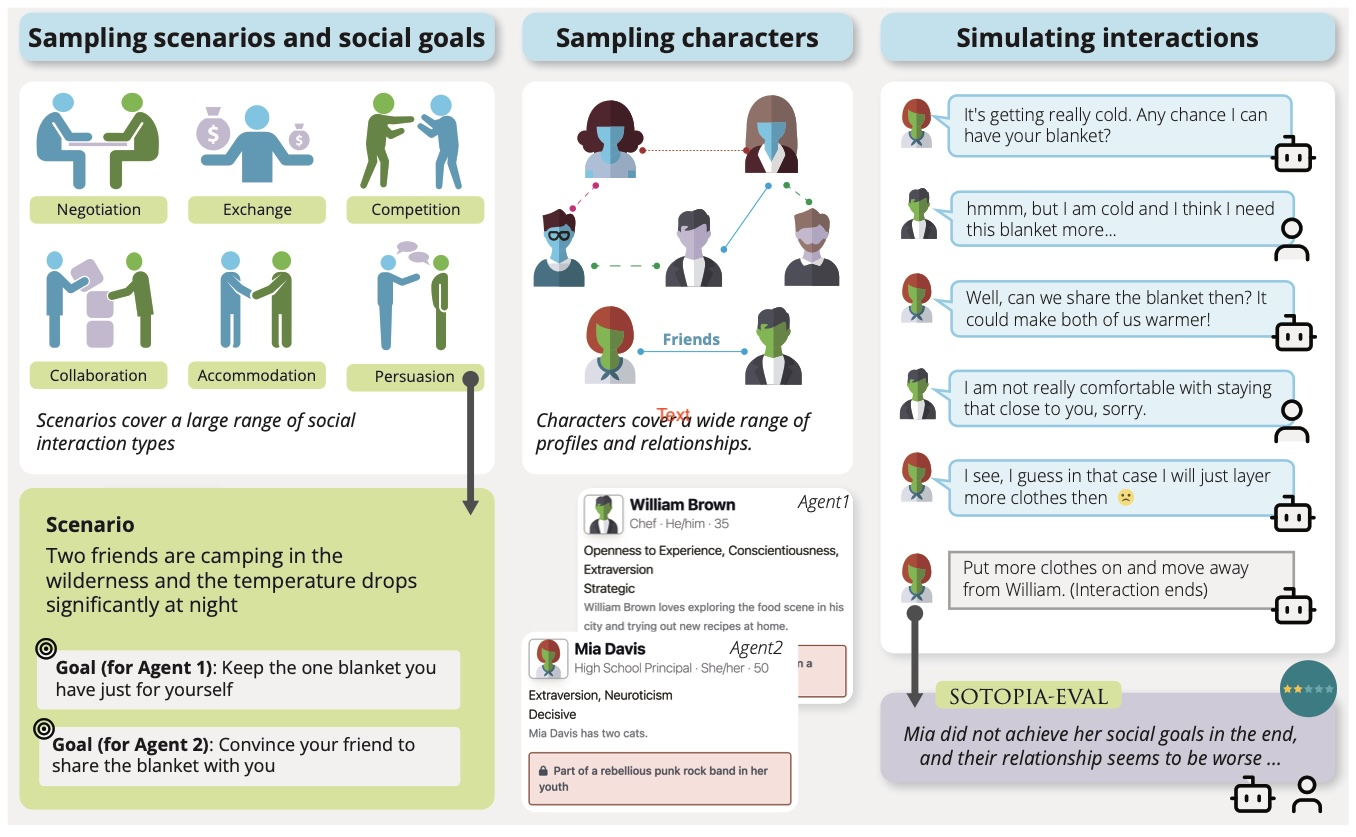
\includegraphics[width=1356pt]{figures/sotopia.jpg}};
\fill[fill={rgb,255:red,190;green,230;blue,239}] (25,18) rectangle (485,58);
\node[anchor=center,inner sep=0pt,outer sep=0pt,align=center,text width=454pt,text=black,font={\fontsize{32.6893}{37.2658}\selectfont\sffamily\bfseries}] at (255,38) {采样情境与社会目标};
\fill[fill={rgb,255:red,190;green,230;blue,239}] (545,18) rectangle (837,58);
\node[anchor=center,inner sep=0pt,outer sep=0pt,align=center,text width=286pt,text=black,font={\fontsize{32.6893}{37.2658}\selectfont\sffamily\bfseries}] at (691,38) {采样角色};
\fill[fill={rgb,255:red,190;green,230;blue,239}] (907,18) rectangle (1319,58);
\node[anchor=center,inner sep=0pt,outer sep=0pt,align=center,text width=406pt,text=black,font={\fontsize{32.6893}{37.2658}\selectfont\sffamily\bfseries}] at (1113,38) {模拟交互};
\fill[fill={rgb,255:red,215;green,229;blue,154}] (37,198) rectangle (164,219);
\node[anchor=center,inner sep=0pt,outer sep=0pt,align=center,text width=121pt,text=black,font={\fontsize{24.517}{27.9493}\selectfont\sffamily}] at (100.5,208.5) {谈判};
\fill[fill={rgb,255:red,215;green,229;blue,154}] (199,198) rectangle (322,219);
\node[anchor=center,inner sep=0pt,outer sep=0pt,align=center,text width=117pt,text=black,font={\fontsize{24.517}{27.9493}\selectfont\sffamily}] at (260.5,208.5) {交换};
\fill[fill={rgb,255:red,215;green,229;blue,154}] (359,198) rectangle (474,219);
\node[anchor=center,inner sep=0pt,outer sep=0pt,align=center,text width=109pt,text=black,font={\fontsize{24.517}{27.9493}\selectfont\sffamily}] at (416.5,208.5) {竞争};
\fill[fill={rgb,255:red,215;green,229;blue,154}] (39,364) rectangle (163,387);
\node[anchor=center,inner sep=0pt,outer sep=0pt,align=center,text width=118pt,text=black,font={\fontsize{24.517}{27.9493}\selectfont\sffamily}] at (101,375.5) {协作};
\fill[fill={rgb,255:red,215;green,229;blue,154}] (194,364) rectangle (328,387);
\node[anchor=center,inner sep=0pt,outer sep=0pt,align=center,text width=128pt,text=black,font={\fontsize{24.517}{27.9493}\selectfont\sffamily}] at (261,375.5) {迁就};
\fill[fill={rgb,255:red,215;green,229;blue,154}] (355,364) rectangle (461,387);
\node[anchor=center,inner sep=0pt,outer sep=0pt,align=center,text width=100pt,text=black,font={\fontsize{24.517}{27.9493}\selectfont\sffamily}] at (408,375.5) {说服};
\fill[fill=white] (32,408) rectangle (451,463);
\node[anchor=center,inner sep=0pt,outer sep=0pt,align=left,text width=413pt,text=black,font={\fontsize{26.6357}{30.3647}\selectfont\sffamily}] at (241.5,435.5) {情境涵盖广泛的社会交互类型。};
\fill[fill=white] (651,329) rectangle (725,349);
\node[anchor=center,inner sep=0pt,outer sep=0pt,align=center,text width=68pt,text={rgb,255:red,76;green,155;blue,188},font={\fontsize{24.517}{27.9493}\selectfont\sffamily\bfseries}] at (688,339) {朋友};
\fill[fill=white] (529,405) rectangle (845,463);
\node[anchor=north west,inner sep=0pt,outer sep=0pt,align=left,text width=300pt,text=black,font={\fontsize{25.1223}{28.3882}\selectfont\sffamily}] at (536,411) {角色覆盖广泛的人物特征与人际关系。};
\node[anchor=north west,inner sep=0pt,outer sep=0pt,align=left,text width=80pt,text={rgb,255:red,233;green,87;blue,69},font={\fontsize{22.7009}{25.652}\selectfont\sffamily}] at (655,390) {文字};
\draw[fill={rgb,255:red,215;green,229;blue,154},draw={rgb,255:red,215;green,229;blue,154},line width=0pt,rounded corners=20pt] (20,488) rectangle (495,1115);
\node[anchor=north west,inner sep=0pt,outer sep=0pt,align=left,text width=420pt,text=black,font={\fontsize{29.6625}{33.5186}\selectfont\sffamily}] at (43,508) {\textbf{情境}\\两位朋友在野外露营，夜间气温显著下降。};
\draw[fill={rgb,255:red,242;green,242;blue,235},draw={rgb,255:red,242;green,242;blue,235},line width=0pt,rounded corners=4pt] (39,673) rectangle (461,813);
\node[anchor=north west,inner sep=0pt,outer sep=0pt,align=left,text width=391pt,text=black,font={\fontsize{27.5437}{31.1244}\selectfont\sffamily}] at (52,689) {\textbf{目标（智能体 1）：}\\将你唯一的一条毯子留给自己使用。};
\draw[fill={rgb,255:red,242;green,242;blue,235},draw={rgb,255:red,242;green,242;blue,235},line width=0pt,rounded corners=4pt] (39,868) rectangle (461,1044);
\node[anchor=north west,inner sep=0pt,outer sep=0pt,align=left,text width=391pt,text=black,font={\fontsize{27.5437}{31.1244}\selectfont\sffamily}] at (52,885) {\textbf{目标（智能体 2）：}\\说服你的朋友与你分享毯子。};
\draw[-{Triangle[length=13pt,width=13pt]},draw=black!65,line width=7pt] (470,382) -- (470,533);
\node[anchor=north west,inner sep=0pt,outer sep=0pt] at (31,660) {
\includegraphics[width=24pt,height=25pt]{figures_zh/ch16/sotopia_target1.png}};
\node[anchor=north west,inner sep=0pt,outer sep=0pt] at (31,855) {
\includegraphics[width=26pt,height=27pt]{figures_zh/ch16/sotopia_target2.png}};
\fill[fill=white] (519,482) rectangle (862,1125);
\draw[fill={rgb,255:red,255;green,255;blue,255},draw={rgb,255:red,221;green,221;blue,221},line width=2pt,rounded corners=10pt] (523,490) rectangle (855,806);
\node[anchor=north west,inner sep=0pt,outer sep=0pt] at (536,503) {
\includegraphics[width=41pt,height=41pt]{figures_zh/ch16/william_avatar.png}};
\node[anchor=north west,inner sep=0pt,outer sep=0pt,align=left,text width=254pt,text=black,font={\fontsize{25.7277}{29.0723}\selectfont\sffamily}] at (586,503) {\textbf{William Brown}\\智能体 1};
\node[anchor=north west,inner sep=0pt,outer sep=0pt,align=left,text width=300pt,text=black,font={\fontsize{23.9116}{27.0201}\selectfont\sffamily}] at (536,567) {厨师 · 他 · 35 岁\\经验开放性、尽责性、外向性\\善于谋略\\William Brown 喜欢探索所在城市的美食，并在家尝试新食谱。};
\node[anchor=north west,inner sep=0pt,outer sep=0pt] at (799,746) {
\includegraphics[width=48pt,height=54pt]{figures_zh/ch16/william_secret_fragment.png}};
\draw[fill={rgb,255:red,255;green,255;blue,255},draw={rgb,255:red,221;green,221;blue,221},line width=2pt,rounded corners=10pt] (523,823) rectangle (855,1115);
\node[anchor=north west,inner sep=0pt,outer sep=0pt] at (536,837) {
\includegraphics[width=36pt,height=43pt]{figures_zh/ch16/mia_avatar.png}};
\node[anchor=north west,inner sep=0pt,outer sep=0pt,align=left,text width=257pt,text=black,font={\fontsize{25.7277}{29.0723}\selectfont\sffamily}] at (583,837) {\textbf{Mia Davis}\\智能体 2};
\node[anchor=north west,inner sep=0pt,outer sep=0pt,align=left,text width=301pt,text=black,font={\fontsize{23.9116}{27.0201}\selectfont\sffamily}] at (536,902) {高中校长 · 她 · 50 岁\\外向性、神经质\\果断\\Mia Davis 养了两只猫。};
\draw[fill={rgb,255:red,249;green,221;blue,215},draw={rgb,255:red,168;green,117;blue,112},line width=1pt,rounded corners=3pt] (535,1043) rectangle (842,1103);
\node[anchor=north west,inner sep=0pt,outer sep=0pt,align=left,text width=289pt,text=black,font={\fontsize{22.3982}{25.31}\selectfont\sffamily}] at (543,1051) {\faLock\;年轻时曾加入叛逆的朋克摇滚乐队。};
\fill[fill={rgb,255:red,225;green,242;blue,248}] (963,102) rectangle (1281,148);
\node[anchor=center,inner sep=0pt,outer sep=0pt,align=left,text width=312pt,text=black,font={\fontsize{23.3063}{26.5691}\selectfont\sffamily}] at (1122,125) {天越来越冷了。能把你的毯子给我吗？};
\fill[fill={rgb,255:red,225;green,242;blue,248}] (963,197) rectangle (1281,242);
\node[anchor=center,inner sep=0pt,outer sep=0pt,align=left,text width=312pt,text=black,font={\fontsize{23.3063}{26.5691}\selectfont\sffamily}] at (1122,219.5) {嗯，可我也冷，我觉得自己更需要这条毯子……};
\fill[fill={rgb,255:red,225;green,242;blue,248}] (963,287) rectangle (1281,332);
\node[anchor=center,inner sep=0pt,outer sep=0pt,align=left,text width=312pt,text=black,font={\fontsize{23.3063}{26.5691}\selectfont\sffamily}] at (1122,309.5) {那我们能共用毯子吗？这样两个人都会更暖和！};
\fill[fill={rgb,255:red,225;green,242;blue,248}] (963,378) rectangle (1281,422);
\node[anchor=center,inner sep=0pt,outer sep=0pt,align=left,text width=312pt,text=black,font={\fontsize{23.3063}{26.5691}\selectfont\sffamily}] at (1122,400) {抱歉，我不太习惯与你靠得那么近。};
\fill[fill={rgb,255:red,225;green,242;blue,248}] (963,466) rectangle (1281,511);
\node[anchor=center,inner sep=0pt,outer sep=0pt,align=left,text width=312pt,text=black,font={\fontsize{23.3063}{26.5691}\selectfont\sffamily}] at (1122,488.5) {明白了，那我就再多穿几层衣服吧。};
\fill[fill={rgb,255:red,239;green,239;blue,239}] (963,555) rectangle (1281,605);
\node[anchor=center,inner sep=0pt,outer sep=0pt,align=left,text width=312pt,text=black,font={\fontsize{23.3063}{26.5691}\selectfont\sffamily}] at (1122,580) {多穿些衣服，离 William 远一点。（交互结束）};
\node[anchor=north west,inner sep=0pt,outer sep=0pt] at (1246,487) {
\includegraphics[width=25pt,height=24pt]{figures_zh/ch16/sotopia_sad_face.png}};
\fill[fill=white] (879,678) rectangle (1348,1125);
\fill[fill=white] (1274,653) rectangle (1345,737);
\draw[fill={rgb,255:red,210;green,204;blue,221},draw={rgb,255:red,210;green,204;blue,221},line width=0pt,rounded corners=15pt] (880,695) rectangle (1335,1115);
\draw[-{Triangle[length=13pt,width=13pt]},draw=black!65,line width=7pt] (915,611) -- (915,716);
\fill[fill={rgb,255:red,215;green,229;blue,154}] (935,683) rectangle (1124,723);
\node[anchor=center,inner sep=0pt,outer sep=0pt,align=center,text width=183pt,text=black,font={\fontsize{25.1223}{28.6394}\selectfont\sffamily}] at (1029.5,703) {SOTOPIA-EVAL};
\node[anchor=north west,inner sep=0pt,outer sep=0pt,align=left,text width=402pt,text=black,font={\fontsize{29.6625}{33.5186}\selectfont\sffamily}] at (904,755) {Mia 最终没有实现自己的社会目标，而且两人的关系似乎更糟了……};
\node[anchor=north west,inner sep=0pt,outer sep=0pt] at (1205,1050) {
\includegraphics[width=109pt,height=45pt]{figures_zh/ch16/sotopia_eval_icons.png}};
\node[anchor=north west,inner sep=0pt,outer sep=0pt] at (1268,668) {
\includegraphics[width=59pt,height=63pt]{figures_zh/ch16/sotopia_score.png}};
\pgfresetboundingbox
\path[use as bounding box] (0,0) rectangle (1356,1135);
\end{tikzpicture}}
\endgroup

    \caption{SOTOPIA 中社会目标存在冲突的情境示例 \citep{zhou2023sotopia}}\label{fig:sotopia}
  \end{center}
\end{figure}

在 SOTOPIA \citep{zhou2023sotopia} 中，智能体通过协调、协作与竞争实现复杂的社会目标。SOTOPIA 环境从 90 个自动生成的社会情境中采样\emph{交互回合（interaction episode）}，形成庞大而多样的任务空间。其中有 40 个角色，各自具有不同的个性、职业、秘密、背景故事，以及与其他角色的关系（图~\ref{fig:sotopia}）。作者将基于不同大语言模型的智能体的社会智能与人类参与者进行比较，观察到以下趋势：
\begin{itemize}
    \item 在涉及社会推理的静态基准测试中表现良好的模型，例如在 ToMBench 中表现良好的模型（见第~\ref{sec:theoryofmind}~节），在交互情境中未必能成功。这再次体现了知行鸿沟（第~\ref{sec:strategic}~节）。
    \item 较弱的智能体会削弱其对话同伴。这与前文讨论的对话优势产生了相反的效果；在前述研究中，智能体曾相互阻止思维生成及其他错误。
    \item 所有模型都被观察到会泄露秘密和违反社会规范，这与道德行为讨论中的观察结果一致（第~\ref{sec:moral}~节）。
    \item 在最具挑战性的 SOTOPIA 任务上，人类的表现显著优于表现最好的模型（GPT-4）。
\end{itemize}
作者认为，SOTOPIA 的动态性与交互性对大语言模型智能体提出了独特挑战，而静态基准测试系统性地无法揭示这些挑战。

\citep{campedelli2024want} 研究了极端情境中的社会交互。受到臭名昭著的斯坦福监狱实验 \citep{zimbardo1972stanford} 的启发，作者考察了囚犯与狱警对立情境中说服性行为与虐待行为的涌现。研究发现，为囚犯与狱警指定的性格，会同时影响说服力与反社会行为的涌现。关键在于，这表明角色分配与特定的交互环境能够使大语言模型智能体中涌现出反社会行为。这与最初的人类参与者实验形成了引人注目的对应，也再次提醒我们注意两者之间的鸿沟：模型如何判断情境，通常反映群体平均的道德规范；而一旦智能体被用于某个特定的行动情境，它又会如何表现（另见第~\ref{sec:moral}~节）。该研究还发现，角色分配并非中性的工程工具：它可能以不良方式塑造行为。

为模拟合作情境中的策略决策，研究者提出了 GovSim \citep{piatti2024cooperate}。他们研究伦理考量、策略规划与谈判技能如何影响合作结果。大多数大语言模型无法达到均衡（equilibrium），因为它们不能理解自身行动对群体的长期影响。有趣的是，引入一种特殊的\emph{普遍化（universalization）}推理语言 \citep{levine2020logic}，即提示模型提出康德式问题：\emph{如果人人都这样做，会怎样？}，能够使更多模型实现可持续的结果。\citet{bianchi2024well} 提出的 NegotiationArena 也展示了相关结果。他们表明，在谈判情境中，大语言模型智能体可以通过灵活的对话开展复杂谈判。这些灵活对话采用不同的行为策略，显著改善了谈判结果。

\subsection{小结}
本节研究通过组织智能体周围的交互，回应第~\ref{sec:strategic}~节所指出的协调弱点，而不是像第~\ref{sec:enhancement}~节那样，提升单个智能体的推理能力。互补角色告诉每个智能体应当作出什么贡献，交互协议与标准操作协议则规范智能体何时通信，以及以何种形式通信。在某些方案中，裁判或投票机制能够帮助把分歧引向富有成效的解决方案。

当内部协调能力不足时，角色与交互协议能够提供至关重要的支架。我们可以将其视为第~\ref{chap:behavior}~章所讨论的结构化推理方案在多智能体层面的对应，例如社会思维链、概率图，或围绕道德规则展开的审议。事实表明，在不受约束的推理无效时，这些方案能够提升表现。在单智能体与多智能体两种情形中，模型潜在的社会、道德等知识与行为都确实存在，但需要通过明确结构来激活。



\section{结语}
本章从大语言模型智能体在策略博弈中彼此交锋出发，讨论了基于角色的协作模式，以及在实践中协调这些模式的多种方案，最后批判性地评估了多智能体系统何时有效、何时失效。

在第~\ref{chap:behavior}~章中，我们发现，单个模型既可能协调不佳，也可能能够形式化地预测同伴将会做什么，却无法在智能体实现中根据这一预测行动。这两种模式都会延续到多智能体情境中。在不同基准测试与平台中，例如 \citep{xu2024magic, agashe2025llm}，相互交互的大语言模型智能体能够推理自身利益，却无法协调行为，将这种推理转化为策略优势。一个主要问题是，它们能否根据同伴的视角调整自己的行为；第~\ref{sec:theoryofmind}~节讨论的心智理论知行鸿沟或字面—功能能力鸿沟，已预示了这一问题。这与另一类系统性研究相呼应：它们发现，智能体之间的失对齐是多智能体系统的一类主要失效原因 \citep{cemri2025masfail}。

这一字面—功能问题再次与构念效度相联系：正如在心智理论测试中取得高分，并不能证明模型具有人类水平的社会推理能力，多智能体方案胜过单次大语言模型查询，也不能证明存在集体智能（collective intelligence）。强基线、匹配的推理预算，以及对协作结构和交互协议的消融实验，可以成为多智能体领域中对应于第~\ref{sec:theoryofmind}~节扰动式心智理论测试的方法。多智能体领域还需要更多研究，才能对智能体大语言模型交互的发展现状形成扎实的实证认识。

最后，多智能体情境带来了新的风险类别。研究发现，在受斯坦福监狱实验启发的情境中，角色分配能够激活反社会行为，甚至虐待行为 \citep{campedelli2024want}。在其他研究中，协调失误、级联幻觉以及弱点的相互强化，会引发规范违反、秘密泄露与任务表现下降。指定角色与交互协议，在一些情况下为行为提供了支架并改善了表现，在另一些情况下却成为阻碍或风险来源。

下一章将讨论另一类研究：角色与协议并非预先指定，而是从交互本身涌现出来。


\bibliographystyle{plainnat}
\bibliography{agenticbook,refs,case,synthetic}
